
\chapter{Latex-Beispiele}
\label{chap:bsp}

\section{Aulistungen}

\begin{itemize}
	\item \textit{Kursiv} Text 1
	\item \textbf{Fett}  
	\item \texttt{TT} 
\end{itemize}

Dasselbe durchnumeriert:

\begin{enumerate}
	\item \textit{Kursiv} Text 1
	\item \textbf{Fett}  
	\item \texttt{TT} 
\end{enumerate}

\newpage
\section{Tabellen}

Eine Tabelle mit Testdaten:


\begin{table}[H]
	\begin{center}
		\begin{tabular}{lrrrrr}\hline\hline
			\multicolumn{1}{l}{\textbf{position}}&
			\multicolumn{1}{c}{\textbf{mean}}&
			\multicolumn{1}{c}{\textbf{median}}&
			\multicolumn{1}{c}{\textbf{sd}}&
			\multicolumn{1}{c}{\textbf{min}}&
			\multicolumn{1}{c}{\textbf{max}}
			\\ \hline
			\textbf{6}&$6.89$&$5.61$&$ 7.29$&$0.31$&$160.12$\\
			\textbf{9}&$5.35$&$4.39$&$ 4.94$&$0.18$&$ 76.40$\\
			\textbf{12}&$8.70$&$6.96$&$10.72$&$0.15$&$239.88$\\
			\textbf{13}&$9.01$&$7.54$&$ 7.60$&$0.15$&$138.86$\\
			\textbf{15}&$8.18$&$6.99$&$ 6.86$&$0.16$&$117.26$\\
			\textbf{16}&$5.26$&$4.42$&$ 4.99$&$0.08$&$110.21$\\
			\textbf{17}&$5.87$&$4.79$&$ 6.13$&$0.15$&$ 98.88$\\
			\textbf{36}&$8.21$&$6.72$&$ 7.58$&$1.36$&$122.35$\\
			\textbf{42}&$6.77$&$5.93$&$ 6.98$&$1.72$&$123.72$\\
			\textbf{43}&$6.27$&$5.53$&$ 3.21$&$0.57$&$ 35.69$\\
			\hline
		\end{tabular}
	\end{center}
	\caption{Eine Tabelle mit Testdaten} 
	\label{tabelle:test}
\end{table}

Sprachen wie z.B. \textbf{R} können Latex-Tabellen exportieren, sie müssen also nicht immer so aufwändig formatiert werden.			


\section{Abbildungen}

\begin{figure}[H]
	%\centering
	\hspace*{-1.5cm}
	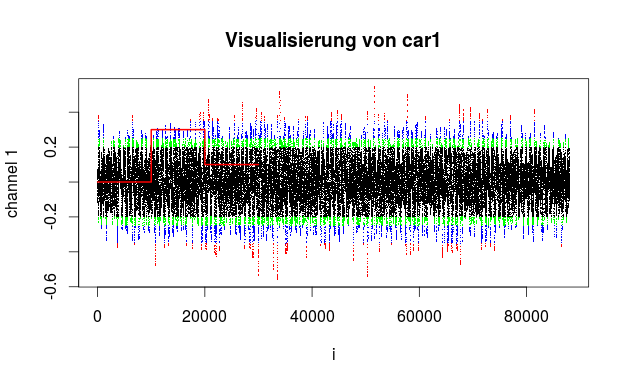
\includegraphics[width=512pt,height=280pt]{figures/bsp.png}
	\caption{Ein Beispiel für ein Bild}
	\label{bild:beispiel}
\end{figure}


\section{Quellcode}

Quellcode wird automatisch (mit der Möglichkeit die Sprache anzugeben) formatiert und in das Listings-Verzeichnis gegeben:

\subsection{Java-Code}

\begin{lstlisting}[style=Java, caption={Java-Beispiel}, captionpos=b]
	int i = 1;
	float f = 2;
	System.out.printf("Int-Z %d Float-Z: 52f",i ,f );
\end{lstlisting} 


\subsection{Python-Code}

\begin{lstlisting}[style=Python, caption={Python-Beispiel}, captionpos=b]
	#Hier ein kleines Beispiel in Python
	lower = 0
	upper = 10
	for i in range(lower,upper):
	print(i)
\end{lstlisting} 


\subsection{Lesen von Dateien}

Es kann auch direkt von Dateien gelesen werden:

\lstinputlisting[style=Java, label={java_bsp}, caption={Java-Beispiel von Datei}, captionpos=b]{sourcecode/First.java}

oder noch ein Beispiel in Python:
\lstinputlisting[style=python, label={python_bsp}, caption={Python-Beispiel von Datei}, captionpos=b]{sourcecode/Second.py}

\section{Referenzen}

Beispiele für die Verwendung von Referenzen: 

\begin{itemize}
	\item Wie in Tabelle ~\ref{tabelle:test} auf Seite \pageref{tabelle:test} ersichtlich... 
	\item Wir sind im Kapitel ~\ref{chap:bsp}
	\item In Zeile 2 im Listing ~\ref{java_bsp} 
\end{itemize}


\section{Zitate}


Hier das Zitat eines Buches: \cite{couper2001} Wird alles automatisch mit  bibtex erledigt.